\chapter{Experiments}
\label{chap:3}
\section{Experimental setup}
\subsection{Methods studied}
So far, we have seen some methods for brain network classification. Now we are going to describe the experiments done with some of them, to evaluate their performance in a more general setting. This means that the experiments are done with other brain networks datasets. In particular, the methods we are going to experiment are four:
\begin{itemize}
	\item Explainable Classification of Brain Networks via Contrast Subgraphs \ref{par:1};
	\item Unsupervised Network Embedding for Graph Visualization, Clustering and Classification \ref{par:2};
	\item Network Classification with Application to Brain Connectomics \ref{par:3};
	\item Stable Biomarker Identification for Predicting Schizophrenia in the Human Connectome \ref{par:4}.
\end{itemize}
To make a recap and have in mind what we are studying, we will briefly summarize what they do. The first two methods are in the family of statistical fingerprints, the second two in Machine learning. 
\vspace{0.5cm}

The first in the list aims to extract a constrast-subgraph, a set of vertices whose induced subgraph is dense in the summary graph of the condition group, and sparse in the summary graph of the control group. To make classification they calculated the number of edges of the subgraph induced by the contrast subgraphs (ASD-TD and TD-ASD) for each patient. They made classification with these two features and an SVM.
\vspace{0.5cm}

In Unsupervised network embedding, they train an autoecoder neural network that construct a feature space for each graph in input. These features, composed of embedding vectors, will be the input of a classification function. 
\vspace{0.5cm}

Network Classification is given us like a library of the programming language R. Their aim is to find nodes or subnetworks with good discriminative power, meaning that they want to select only the most informative nodes and edges. To capture structural assumptions on these informative edges, they focus on convex structured sparsity penalties, with convex optimization. 
\vspace{0.5cm}

In Stable Biomarkers identification they perform an automatic feature selection procedure to identify biomarkers that will be used to classify brain networks. In this case classify people affected by schizophrenia. To make classification they also design a RFE-SVM classifier. 

\subsection{Datasets used}
The principle datasets are four big ones, from which are extracted other ones. The main four are:
\begin{itemize}
	\item \textbf{ABIDE} (Autism Brain Imaging Data Exchange) \cite{Cameron2013TheNB}, is a collaboration of 16 international imaging sites that have aggregated and are openly sharing neuroimaging data from 539 individuals suffering from ASD (autism) and 573 typical controls. These 1112 datasets are composed of structural and resting state functional MRI data along with an extensive array of phenotypic information. All data are preprocessed and different types of preprocessing are described in the web site.
	\item \textbf{MTA} (Multimodal Treatment of Attention Deficit Hyperactivity Disorder) \cite{mta}, datasets from a subset of MTA participants at 6 sites, both with and without childhood ADHD, who were studied as part of a follow-up multimodal brain imaging examination. The principal aim of the effort was to investigate the effect of cannabis use among adults with a childhood diagnosis of ADHD. The study was a 2x2 design of those with/without ADHD and those who did/did not regularly use cannabis.
	\item \textbf{HCP} (Human Connectome Project) \cite{Woolrich2001TemporalAI}, includes high-resolution scans from young healthy adult twins and non-twin siblings (ages 22-35) using four imaging modalities: structural images, resting-state fMRI (rfMRI), task-fMRI (tfMRI), and high angular resolution diffusion imaging (dMRI). Behavioural and other individual subject measure data are included on all subjects. 
	\item \textbf{Schizophrenia} \cite{schizo}, is a dataset acquired from approximately 100 patients with schizophrenia and 100 age-matched controls during rest as well as several task activation paradigms targeting a hierarchy of cognitive constructs. Neuroimaging data include structural MRI, functional MRI, diffusion MRI, MR spectroscopic imaging, and magneto-encephalography.
\end{itemize}

The datasets have been extracted from ABIDE are four, \textit{Children}, that includes patients which are at most 9 years, \textit{Adolescents}, individuals between 15 and 20 years old, \textit{EyesClosed}, with people that performed their fMRI with their eyes closed, and \textit{Male}, considering only male subjects. These had been already extracted by T. Lanciano et al \cite{lanciano2020cs}, and kindly given to me to make experiments. We want to stress that, except from ABIDE and \textit{children}, the others are only in binary form, meaning that they have not weighted edges, but only zeros and ones (1 if there is a connection, 0 if there is not).
\vspace{0.5cm}

From HCP dataset we though that could be interesting to divide male and female patients, dataset that we will call hcp\_gender, to see if they are in some way different in their brain connections, like in some other papers described in \ref{chap:2}. 
\vspace{0.5cm}

From MTA we exstracted two datasets, one that divides between patients with ADHD and patients without it, that we will call \textit{mta}, and a dataset that distiguish people that make use of cannabis, from people that do not use it, that we will call \textit{mta\_cannabis}.
\vspace{0.5cm}

At the end we have nine datasets: ABIDE, Children, Adolescents, EyesClosed, Male, mta, mta\_cannabis, Schizophrenia and hcp\_gender. 
\vspace{0.5cm}

It is important to specify that each patient is represented by an adjacency matrix contained in a .csv file.

\subsection{Code}
All the experiments were launched with the program Anaconda. We start with an environment of Python 3.5, but some of the methods were written in Python 2.7, so we switched to an Anaconda environment with Python 2.7 when requested from the method.
\vspace{0.5cm}

To make the experiments easier to perform, was implemented a python script at which can be specified, as input arguments, which method we want to evaluate, which dataset to use and even if the data must be weighted or binary, meaning that one can choose to have weighted edges of the network, or binary ones. Obviously, the dataset that are already in binary form, will not be studied in weighted form, but will be left as they are, except from the preprocessing.
\vspace{0.5cm}

After a method has been runned there is the classification part. The classification is done for only two of the methods we take in consideration. These are \textit{Explainable Classification of Brain Networks via Contrast Subgraphs} \cite{lanciano2020cs} and \textit{Unsupervised Network Embedding for Graph Visualization, Clustering and Classification} \cite{GutierrezUn}, because, as said in their summary explanation, what we extract form them are some features of the graphs in input, and for this reason we have to design a classification for them. The other two methods have their own classification in the code, and we though it was not reasonable to use a different one.
\vspace{0.5cm}

Our classifier is designed with the grid search function of the Python library sklearn, to find the best parameters for each method. We used a cross-validation of 5/10 folds, repeated 5 times. To split the dataset we choose to have 80\% of train set and 20\% of test set. Then from the best parameters found, we make predictions and evaluate the performance with \textbf{accuracy}. The accuracy is calculated directly from the grid search function for each loop of the cross-validation, so we take the mean of all the values. 
\vspace{0.5cm}

All datasets have their own preprocess, made from who released the data. We also added some data modification before to give the datasets to the algorithms. First of all is checked if the values of the diagonal of each matrix were zeros, if not they are corrected, because we do not want to consider each ROI connected to itself, so like an edge. Then, for each adjacency matrix we calculated the 0.2 quantile and 0.8 quantile, to leave out all the values of the edges bigger than the 0.2 quantile and lower than the 0.8 quantile. We do that because we want to consider only the most relevant nodes, and the ones that are in the middle are oblviosly less informative. This is done for all datasets. 
\vspace{0.5cm}

Now, as we said, we could choose if transform the datasets in binary edged or leave them with weighted edges. If it is chosen to transform them in binary data, after leaving out the values below and above the quantiles, all the values different from zero are transformed in ones, even the negative values.

\section{Results}
Now we are going to show the results of each method.
\vspace{0.5cm}

\subsection{Results of Explainable Classification of Brain Networks via Contrast Subgraphs}

With the code taken from the work of Lanciano et al \cite{lanciano2020cs} we extract the two contrast-subgraphs ASD-TD and TD-ASD. Then we calculate the subgraphs induced by the two contrast-subgraphs on each patient. For each subgraph obtained we count the number of edges. In this way we have two features (columns), one is the number of edges induced by ASD-TD for each patient, and the other is the number of edges induced by TD-ASD for each patient.  Each patient is represented by a row. We give these features to the classifier described in the previous section, designed by us. This procedure is done for each dataset, and for each dataset is done for weighted data and binary data. The parameter $\alpha$ is obtained by taking the percentile of the summary graphs of the two study groups. The percentile is decided through meny experiments, we tried with the percentiles $ = {70, 75, 80, 85, 90, 95}$ for each dataset.
\vspace{0.5cm}

Each experiment is repeated ten times, in order to take the mean of all the accuracies, and the standard deviation. The results obtained with each dataset is shown in Table \ref{tab:c-s}. We can see that the best result with this method is given with the dataset \textit{mta} both in binary and weighted form. The running time to extract the contrast-subgraphs is very low, only few seconds, and the running time to make classification is at most 16 minutes.
\vspace{0.5cm}
\begin{table}
	\centering
	\begin{tabular}{c|l|c} 
		\toprule
		& \multicolumn{1}{c|}{b} & w                \\ 
		\midrule
		\textbf{children}      & 0.51 $\pm$ 0.04        & 0.49 $\pm$ 0.08  \\
		\textbf{adolescents}   & 0.53 $\pm$ 0.03        & 0.53 $\pm$ 0.03  \\
		\textbf{eyesclosed}    & 0.54 $\pm$ 0.09        & 0.54 $\pm$ 0.09  \\
		\textbf{male}          & 0.51 $\pm$ 0.07        & 0.51 $\pm$ 0.07  \\
		\textbf{ABIDE}         & 0.52 $\pm$ 0.03        & 0.52 $\pm$ 0.06  \\
		\textbf{mta}           & \textbf{0.69 $\pm$ 0.03}        & \textbf{0.69 $\pm$ 0.02}  \\
		\textbf{hcp\_gender}   & 0.53 $\pm$ 0.11        & 0.53 $\pm$ 0.02  \\
		\textbf{schizophrenia} & 0.54 $\pm$ 0.05        & 0.51 $\pm$ 0.06  \\
		\textbf{mta\_cannabis} & 0.47 $\pm$ 0.04        & 0.55 $\pm$ 0.10 
	\end{tabular}
	\caption{Results of Contrast-subgraph method with each dataset.}
	\label{tab:c-s}
\end{table}

It is interesting to see how change the number of edges induced by both the contrast-subgraphs, depending on the class of the patient. In the scatterplot of Figure \ref{fig:diagram19} are reported these features for the best result obtained with this method, so with dataset mta and $ \alpha = 0.05 $. We can notice that the majority of tipically developed patients have more edges induced by contrast subgraph ASD-TD than patients affected by Autism,. Also, we can see the diagonal line that should represent the division between the two classes of patients. Our is not very precise, and we can see that even from the accuracy result, that is 69\%.

\begin{figure}[htbp]
	\centering
	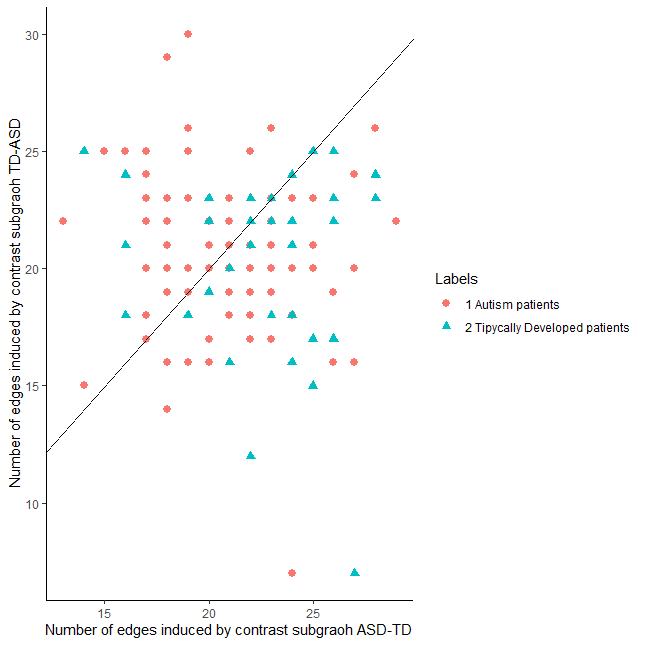
\includegraphics[scale=0.5]{Immagini/scatterplot_cs_mta.png}
	\caption{Scatterplot of number of edges induced by the contrast subgraphs to mta dataset. At $x$-axis there the number of edges induced by the contrast subgraph ASD-TD, while at $y$-axis the once induced by the contrast subgraph TD-ASD, on each patient.}
	\label{fig:diagram19}
\end{figure}


\subsection{Results of Unsupervised Network Embedding for Graph Visualization, Clustering and Classification}

The output we have from \textit{Unsupervised Network Embedding} is an embedded vector for each patient. The embedded vector contains 1024 values, so we will have a matrix in which each row corresponds to a patient, and the columns are the values of the embedded vector of each patient. Obviously, each dataset is studied separately and each one has different extracted features. We give the features to our classifier, and repeat the experiment ten times for each dataset, to take at the end the mean of all accuracies and the standard deviation.
\vspace{0.5cm}

The results for each dataset are shown in Table \ref{tab:embs}. From that we can see that this method worked better with the dataset mta in weighted form, so leaving the edges weighted, and with dataset schizophrenia in binary form. In general we can say that datasets in binary form have slightly better results. This algorithm has five parameters that can be changed: \textit{number of epochs}, \textit{batch size}, \textit{embedding size}, \textit{learning rate} and the \textit{noise} to apply to data. We made many tests with different parameters to find the best combination for each dataset.
\vspace{0.5cm}

\begin{table}
	\centering
	\begin{tabular}{c|l|c} 
		\toprule
		& \multicolumn{1}{c|}{b} & w                \\ 
		\midrule
		\textbf{children}      & 0.55 $\pm$ 0.05        & 0.56 $\pm$ 0.05  \\
		\textbf{adolescents}   & 0.59 $\pm$ 0.07        & 0.59 $\pm$ 0.07  \\
		\textbf{eyesclosed}    & 0.57 $\pm$ 0.04        & 0.57 $\pm$ 0.04  \\
		\textbf{male}          & 0.56 $\pm$ 0.02        & 0.56 $\pm$ 0.02  \\
		\textbf{ABIDE}         & 0.56 $\pm$ 0.01        & 0.57 $\pm$ 0.05  \\
		\textbf{mta}           & \textbf{0.67 $\pm$ 0.03}        & 0.64 $\pm$ 0.09  \\
		\textbf{hcp\_gender}   & 0.64 $\pm$ 0.08        & 0.63 $\pm$ 0.02  \\
		\textbf{schizophrenia} & 0.63 $\pm$ 0.03        & \textbf{0.67 $\pm$ 0.01}  \\
		\textbf{mta\_cannabis} & 0.58 $\pm$ 0.03        & 0.56 $\pm$ 0.09 
	\end{tabular}
	\caption{Results of Unsupervised network embedding method with each dataset.}
	\label{tab:embs}
\end{table}

The running time to extract the features depends most of all on the number of epochs and length of the data, anyway it is not very high, more and less 15 minutes. Even the classification part does not take long, the maximum time, with both extracting the features and classification, is 2 hours, but the mean of the total runtime between all the datasets is 30 minutes.

\subsection{Results of Network Classification with Application to Brain Connectomics}

In this work is implemented also the classification. It is written in R code, and, to compute the accuracy score, we were able to extract the predicted values and the true values. The main function is \textit{graphclass()}, and has three parameters to try and tune, that are lamba $\lambda$, rho $\rho$ and gamma $\gamma$. As in the previous experiments, we run the algorithm 10 times for each dataset, then compute the mean of all accuracies and the standard deviation. The results for all the datasets are in Table \ref{tab:graphclass}. The best score is with the dataset hcp\_gender, for which the best parameters are $\lambda = 10^{-4} $, $\rho = 1$ and $\gamma = 10^{-5}$. 
\vspace{0.5cm}

The mean of the running time is 5 minutes, anyway it is not more than 11 minutes, depending on the length of the data. 

\begin{table}
	\centering
	\begin{tabular}{c|l|c} 
		\toprule
		& \multicolumn{1}{c|}{b} & w                \\ 
		\midrule
		\textbf{children}      & 0.59 $\pm$ 0.09        & 0.54 $\pm$ 0.07  \\
		\textbf{adolescents}   & 0.61 $\pm$ 0.05        & 0.61 $\pm$ 0.05  \\
		\textbf{eyesclosed}    & 0.55 $\pm$ 0.05        & 0.55 $\pm$ 0.05  \\
		\textbf{male}          & 0.61 $\pm$ 0.02        & 0.61 $\pm$ 0.02  \\
		\textbf{ABIDE}         & 0.61 $\pm$ 0.04        & 0.58 $\pm$ 0.03  \\
		\textbf{mta}           & 0.71 $\pm$ 0.03        & 0.68 $\pm$ 0.02  \\
		\textbf{hcp\_gender}   & \textbf{0.77 $\pm$ 0.01}        & 0.71 $\pm$ 0.03  \\
		\textbf{schizophrenia} & 0.58 $\pm$ 0.09        & 0.59 $\pm$ 0.06  \\
		\textbf{mta\_cannabis} & 0.57 $\pm$ 0.07        & 0.59 $\pm$ 0.12 
	\end{tabular}
\caption{Results of Network classification method with each dataset.}
\label{tab:graphclass}
\end{table}

\subsection{Results of Stable Biomarker Identification for Predicting Schizophrenia in the Human Connectome}

As the previous model, even \textit{Stable Biomarkers Identification} has already in the code the classification part. The results that we have in output is a .mat file, where are stored all the accuracies computed at each step of the outer cross-validation (see \ref{par:4}). Each accuracy corresponds to the mean of all accuracies evaluated within the inner cross-validation, in which each step corresponds a certain percentage of features. Each accuracy has also the corrispondent standard deviation. We show the best accuracy computed, even if this means that each dataset could have the best result with a different number of features. Regarding the data, they want to study functional, structural and multimodal data. We only have functional networks, so we will make evaluation only on this kind of data modality. Also, at the end, they evaluate the robustness of the selected features, the trade-off between accuracy and stability, and identify the set of brain regions engaged in the discrimination of patients. In our work, we will only stop at classification evaluation. From Table \ref{tab:biomarkers} we can see all the results obtained with each dataset. As we can see, we have the best result with this method with the dataset \textit{schizophrenia}, in binary form.
\vspace{0.5cm}

\begin{table}
	\centering
	\begin{tabular}{c|l|c} 
		\toprule
		& \multicolumn{1}{c|}{b} & w                \\ 
		\midrule
		\textbf{children}      & 0.59 $\pm$ 0.09        & 0.54 $\pm$ 0.07  \\
		\textbf{adolescents}   & 0.61 $\pm$ 0.05        & 0.61 $\pm$ 0.05  \\
		\textbf{eyesclosed}    & 0.55 $\pm$ 0.05        & 0.55 $\pm$ 0.05  \\
		\textbf{male}          & 0.61 $\pm$ 0.02        & 0.61 $\pm$ 0.02  \\
		\textbf{ABIDE}         & 0.61 $\pm$ 0.04        & 0.58 $\pm$ 0.03  \\
		\textbf{mta}           & 0.71 $\pm$ 0.03        & 0.68 $\pm$ 0.02  \\
		\textbf{hcp\_gender}   & 0.77 $\pm$ 0.01        & 0.71 $\pm$ 0.03  \\
		\textbf{schizophrenia} & 0.58 $\pm$ 0.09        & 0.59 $\pm$ 0.06  \\
		\textbf{mta\_cannabis} & 0.57 $\pm$ 0.07        & 0.59 $\pm$ 0.12 
	\end{tabular}
\caption{Results of Stable biomarkers identification method with each dataset.}
\label{tab:biomarkers}
\end{table}

The running time of this implementation is very high, it depends on the dimention of the dataset, but it takes from six to eight ours to end. This is because they try with many features percentage, and for each one the accuracy is evaluated many times. We recall that this is the description of their designed an RFE-SVM, meaning that they compute the accuracy for different percentage of features taken. For this reason it is interesting to see how the accuracy changes according to the features percentage. In their pubblication they already showed some plots to evaluate this attribute. We took the same plot, the one already written from them in a python script, and adapted it to our results. This is shown in Figure \ref{fig:diagram20}. The graph shows us that in this case the accuracy does not change much according to features percentage, still more features we consider, more the accuracy is high, even if sligthly. 

\begin{figure}[htbp]
	\centering
	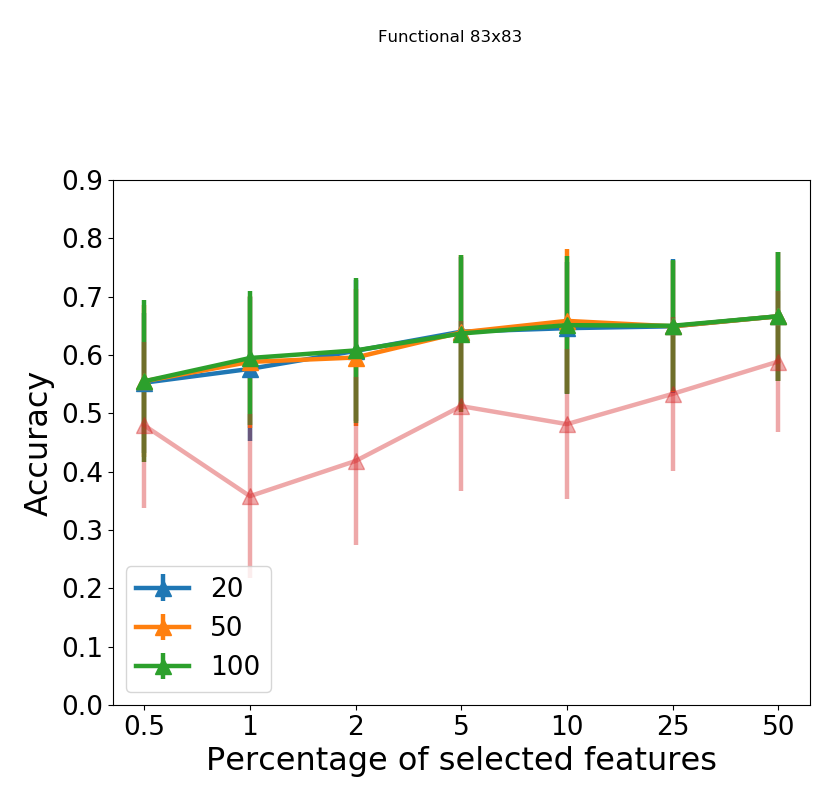
\includegraphics[scale=0.5]{Immagini/fc_83_schizo.png}
	\caption{Graph representing the accuracy according to the percentage of features selected to make classification.}
	\label{fig:diagram20}
\end{figure}


\section{Discussion}

We can see the summary of all the results mentioned in this chapter in Table \ref{tab:all_results}. In general, we do not have very hihg results. This could be due to preprocessing and parameters tuning reasons. Anyway, according to our experiments, the methods that have best accuracy are \textit{Stable Biomarkers identification for predicting schizophrenia in Human Connectome} and textit{Network classification with Application to Brain Connectomics}. This means that they are valid tools to make classification on brain networks. 
\vspace{0.5cm}

\begin{table}
\centerline{
\setlength{\tabcolsep}{2.25pt}
\begin{tabular}{c|c|c|c|c|c}
	\multicolumn{1}{c}{}                    &                        & \textbf{Contrast-subgraph}   & \textbf{GraphEmbs}    & \textbf{Biomarkers}   & \textbf{Graphclass}   \\ 
	\midrule
	\multirow{2}{*}{\textbf{children}}      & b                      & 0.50 $\pm$ 0.02 & 0.50 $\pm$ 0.02              &                       &                       \\ 
	\cline{2-6}
	& w                      &                              &                       &                       &                       \\ 
	\midrule
	\multirow{2}{*}{\textbf{adolescents}}   & b                      &                              &                       &                       &                       \\ 
	\cline{2-6}
	& \multicolumn{1}{l|}{w} & \multicolumn{1}{l|}{}        & \multicolumn{1}{l|}{} & \multicolumn{1}{l|}{} & \multicolumn{1}{l}{}  \\ 
	\midrule
	\multirow{2}{*}{\textbf{eyesclosed}}    & b                      &                              &                       &                       &                       \\ 
	\cline{2-6}
	& \multicolumn{1}{l|}{w} & \multicolumn{1}{l|}{}        & \multicolumn{1}{l|}{} & \multicolumn{1}{l|}{} & \multicolumn{1}{l}{}  \\ 
	\midrule
	\multirow{2}{*}{\textbf{male}}          & b                      &                              &                       &                       &                       \\ 
	\cline{2-6}
	& \multicolumn{1}{l|}{w} & \multicolumn{1}{l|}{}        & \multicolumn{1}{l|}{} & \multicolumn{1}{l|}{} & \multicolumn{1}{l}{}  \\ 
	\midrule
	\multirow{2}{*}{\textbf{ABIDE}}         & b                      &                              &                       &                       &                       \\ 
	\cline{2-6}
	& \multicolumn{1}{l|}{w} & \multicolumn{1}{l|}{}        & \multicolumn{1}{l|}{} & \multicolumn{1}{l|}{} & \multicolumn{1}{l}{}  \\ 
	\midrule
	\multirow{2}{*}{\textbf{mta}}           & b                      &                              &                       &                       &                       \\ 
	\cline{2-6}
	& \multicolumn{1}{l|}{w} & \multicolumn{1}{l|}{}        & \multicolumn{1}{l|}{} & \multicolumn{1}{l|}{} & \multicolumn{1}{l}{}  \\ 
	\midrule
	\multirow{2}{*}{\textbf{hcp\_gender}}   & b                      &                              &                       &                       &                       \\ 
	\cline{2-6}
	& \multicolumn{1}{l|}{w} & \multicolumn{1}{l|}{}        & \multicolumn{1}{l|}{} & \multicolumn{1}{l|}{} & \multicolumn{1}{l}{}  \\ 
	\midrule
	\multirow{2}{*}{\textbf{schizophrenia}} & b                      &                              &                       &                       &                       \\ 
	\cline{2-6}
	& \multicolumn{1}{l|}{w} & \multicolumn{1}{l|}{}        & \multicolumn{1}{l|}{} & \multicolumn{1}{l|}{} & \multicolumn{1}{l}{}  \\
	\bottomrule
\end{tabular}
}
\caption{Accuracy results and standard deviation of each method experimented with each dataset.}
\label{tab:all_results}
\end{table}

The accuracy is not the only evaluation that is worth to take in consideration. Obviously it is really important to have right results, in order to use these methods for scientific purpuses. What we think also important to evaluate is the running time. All the algortihms that we evaluated have different running times, we can see them in Figure (...). From this plot we can see how much time the work of Guti\'{e}rrez et al. \cite{GutierrezBio} takes to evaluate all the dataset, and this is not very good if we want to make a diagnosis for a patient. 
\vspace{0.5cm}

Taking in mind the considerations made now, we can say that between the methods we choose to make brain network classification, the best one is \textit{Network classification with Application to Brain Connectomics}, in fact it gives the best results of our experiments and do not take much time to evaluate out datasets.

From these results we can say that even the dataset is important, because it needs to be as good as possible for that method. Here we have several datasets. Most of them have been collected with different machines and technologies. Also, they have been trasformed and preprocessed in different ways. This is the reason why it is important to evaluate each method with the highest amount of datasets, because we want to see how the results change. We can see if some method is more sutable for some kind of mental disease, even if it written that could be used for all mental disorder.
